% Design-space exploration for compute-near-memory systems -- ESWEEK 2026 tutorial
% Build: make   (latexmk -pdf)
\documentclass[aspectratio=169,10pt]{beamer}
\usetheme{metropolis}
\usepackage{booktabs}
\usepackage{tikz}
\usetikzlibrary{positioning,fit,arrows.meta,calc}
\usepackage{fontawesome5}

% The palette the notebooks draw with
\definecolor{cblue}{HTML}{2a78d6}
\definecolor{corange}{HTML}{eb6834}
\definecolor{caqua}{HTML}{1baf7a}
\definecolor{cink}{HTML}{0b0b0b}
\definecolor{cink2}{HTML}{52514e}
\definecolor{cgrid}{HTML}{e3e2dd}
\setbeamercolor{progress bar}{fg=cblue}
\setbeamercolor{alerted text}{fg=corange}
\setbeamercolor{title separator}{fg=cblue}

\newcommand{\notebookframe}[3]{%
  \begin{frame}[standout]
    \Huge Notebook #1\par
    \vspace{.6em}\normalsize #2\par
    \vspace{1.2em}\footnotesize\color{cgrid}#3
  \end{frame}}

\title{Finding a needle in $4\times10^{9}$ configurations}
\subtitle{Design-space exploration for compute-near-memory systems}
\author{Clément Fournier}
\institute{TU Dresden}
\date{ESWEEK 2026}

\begin{document}

\maketitle

% ─────────────────────────────────────────────────────────────────────────
\begin{frame}{Today}
  \begin{columns}[T]
    \column{.55\textwidth}
    \textbf{One question, held for 45 minutes}\par
    \medskip
    \emph{Every configuration costs a simulation, and there are too many to try.
    How do you find a good one --- and how do you know it is good?}
    \bigskip
    \begin{enumerate}
      \item Where the configuration space comes from \hfill\small slides + notebook 1
      \item What the space looks like \hfill\small notebook 2
      \item Searching it on a budget \hfill\small slides + notebook 3
    \end{enumerate}
    \column{.4\textwidth}
    \begin{block}{Open the notebooks now}
      \centering
      \fbox{\parbox{.85\linewidth}{\centering\vspace{2.2em}Binder QR / link\vspace{2.2em}}}\par
      \smallskip\footnotesize Binder takes a minute to start; let it while we do slides.
    \end{block}
  \end{columns}
\end{frame}

% ─────────────────────────────────────────────────────────────────────────
\section{The hardware}

\begin{frame}{Compute near memory, four ways}
  \begin{columns}[T]
    \column{.24\textwidth}\centering
    \fbox{\parbox{.9\linewidth}{\centering\vspace{3em}UPMEM\vspace{3em}}}\par
    \small DPUs in DRAM ranks
    \column{.24\textwidth}\centering
    \fbox{\parbox{.9\linewidth}{\centering\vspace{3em}HBM-PIM\vspace{3em}}}\par
    \small SIMD units per bank
    \column{.24\textwidth}\centering
    \fbox{\parbox{.9\linewidth}{\centering\vspace{3em}SIMDRAM\vspace{3em}}}\par
    \small compute in the cell array
    \column{.24\textwidth}\centering
    \fbox{\parbox{.9\linewidth}{\centering\vspace{3em}UniNDP\vspace{3em}}}\par
    \small the design space of all of them
  \end{columns}
  \bigskip
  \footnotesize Figures: UPMEM (Devaux, HotChips'19), Samsung HBM-PIM (Lee et al., ISCA'21), SIMDRAM (Hajinazar et al., ASPLOS'21), UniNDP (Li et al., HPCA'25).
\end{frame}

\begin{frame}{What they have in common}
  \begin{columns}[T]
    \column{.5\textwidth}
    \begin{itemize}
      \item \textbf{Many small compute nodes} --- thousands, each slow on its own
      \item \textbf{Each owns a slice of memory} --- fast to reach locally, slow or impossible across
      \item \textbf{A hierarchy of levels} --- bank / rank / channel; node-local scratchpad
      \item \textbf{A narrow interface to the host} --- data goes in and out through it
      \item \textbf{Programmable} --- what runs where is a software decision
    \end{itemize}
    \column{.48\textwidth}
    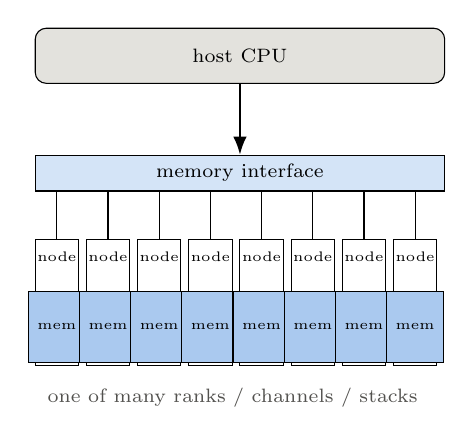
\begin{tikzpicture}[scale=.8, every node/.style={font=\scriptsize}]
      \node[draw, rounded corners, minimum width=5.2cm, minimum height=.7cm, fill=cgrid] (host) {host CPU};
      \node[below=.9cm of host, draw, minimum width=5.2cm, minimum height=.35cm, fill=cblue!20] (bus) {memory interface};
      \draw[-{Latex}, thick] (host) -- (bus);
      \foreach \i in {0,...,7} {
        \node[below=.6cm of bus.south west, anchor=north west, xshift={\i*.65cm}, draw, minimum width=.55cm, minimum height=1.6cm, fill=white] (n\i) {};
        \node[anchor=north] at ([yshift=-.05cm]n\i.north) {\tiny node};
        \node[anchor=south, draw, fill=cblue!40, minimum width=.45cm, minimum height=.9cm] at ([yshift=.05cm]n\i.south) {\tiny mem};
        \draw (bus.south -| n\i) -- (n\i.north);
      }
      \node[below=.15cm of n3.south east, font=\scriptsize\color{cink2}] {one of many ranks / channels / stacks};
    \end{tikzpicture}
  \end{columns}
  \bigskip
  \alert{The consequence:} a kernel is not \emph{run} on such a system, it is \emph{distributed} onto it. How is the design decision.
\end{frame}

% ─────────────────────────────────────────────────────────────────────────
\section{The kernel}

\begin{frame}[fragile]{Our running example: $y = A x$}
  \begin{columns}[T]
    \column{.5\textwidth}
    \begin{align*}
      y_m &= \sum_{k} A_{m,k}\, x_k \\[.5em]
      &\text{for } m \in M,\ k \in K
    \end{align*}
    \medskip
    Two loop dimensions with very different characters:
    \begin{itemize}
      \item $M$ is \textbf{parallel} --- rows are independent
      \item $K$ is a \textbf{reduction} --- splitting it means partial sums to combine
    \end{itemize}
    \column{.46\textwidth}
    \small In Cinnamon's MLIR input:
    \begin{semiverbatim}\scriptsize
#upmem = #upmem.platform<type = v1A,
                          dpus = 64, tasklets = 16>

func.func @gemv(\%A: tensor<1024x1024xi32>,
                \%x: tensor<1024xi32>)
    attributes \{cinm.available_platforms = [#upmem]\} \{
  cinm.compute \{
    cinm.op.gemv \%A, \%x
  \}
\}
    \end{semiverbatim}
    \footnotesize One DRAM rank: 64 DPUs, 16 hardware threads each, 64 MB MRAM and 64 KB WRAM per DPU.
  \end{columns}
\end{frame}

\begin{frame}{Tiling to the memory levels}
  \begin{columns}[T]
    \column{.5\textwidth}
    \centering
    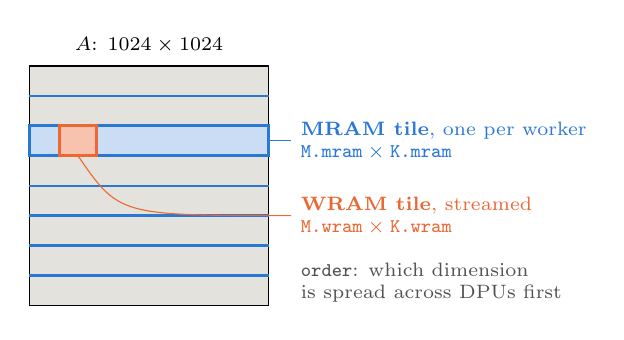
\begin{tikzpicture}[scale=.95, every node/.style={font=\scriptsize}]
      \draw[fill=cgrid] (0,0) rectangle (3.2,3.2);
      \node[anchor=south] at (1.6,3.25) {$A$: $1024 \times 1024$};
      \foreach \i in {1,...,7} \draw[cblue, thick] (0,\i*0.4) -- (3.2,\i*0.4);
      \draw[cblue, very thick, fill=cblue!25] (0,2.0) rectangle (3.2,2.4);
      \draw[corange, very thick, fill=corange!40] (0.4,2.0) rectangle (0.9,2.4);
      % labels, stacked to the right of the matrix
      \node[anchor=west, cblue, align=left] at (3.5,2.2) {\textbf{MRAM tile}, one per worker\\ $\texttt{M.mram} \times \texttt{K.mram}$};
      \draw[cblue] (3.2,2.2) -- (3.5,2.2);
      \node[anchor=west, corange, align=left] at (3.5,1.2) {\textbf{WRAM tile}, streamed\\ $\texttt{M.wram} \times \texttt{K.wram}$};
      \draw[corange] (0.65,2.0) .. controls (1.2,1.2) .. (3.5,1.2);
      \node[anchor=west, cink2, align=left] at (3.5,0.3) {\texttt{order}: which dimension\\ is spread across DPUs first};
    \end{tikzpicture}
    \column{.46\textwidth}
    \textbf{Each choice must satisfy}
    \medskip
    \begin{itemize}\small
      \item tiles divide the extents: $\texttt{M.mram} \mid 1024$, $\texttt{K.mram} \mid 1024$
      \item inner tiles divide outer ones: $\texttt{M.wram} \mid \texttt{M.mram}$, \ldots
      \item one tile per worker:\\ $\dfrac{1024}{\texttt{M.mram}} \cdot \dfrac{1024}{\texttt{K.mram}} = \texttt{dpus} \cdot \texttt{tasklets}$
      \item what the tasklets hold fits: $\le$ MRAM, $\le$ WRAM
      \item DMA granularity: tiles are multiples of 8 bytes
    \end{itemize}
  \end{columns}
  \bigskip
  \centering\small Every arrow in the picture is a parameter; every ``must'' is a constraint.
\end{frame}

\begin{frame}{The hardware knobs are not separate}
  \begin{columns}[T]
    \column{.5\textwidth}
    \textbf{How many DPUs? How many tasklets?}\par
    \medskip
    These look like \emph{platform} decisions --- fix them first, then tile.
    \medskip
    But:
    \begin{itemize}
      \item the tile count must equal the worker count: \\ $\prod (\text{extent}/\text{tile}) = \texttt{dpus}\cdot\texttt{tasklets}$
      \item more tasklets $\Rightarrow$ smaller tiles $\Rightarrow$ more launch overhead per byte
      \item more DPUs $\Rightarrow$ more transfer parallelism, more partial results to gather
    \end{itemize}
    \column{.46\textwidth}
    \begin{alertblock}{Measured on the small space}
      best latency with \texttt{tasklets} = \\
      \begin{tabular}{@{}rrrrr@{}}
        1 & 2 & 4 & \textbf{8} & 16 \\
        8.0 & 4.2 & 2.4 & \textbf{1.6} & 7.8 \\
      \end{tabular}\\[.4em]
      \footnotesize (ms) --- ``use all the threads'' is $5\times$ off.
    \end{alertblock}
    \medskip
    \small On $4096^2$ with 32 ranks the optimum is \textbf{1 tasklet} on all 2048 DPUs. The right knob setting flips with problem size.
  \end{columns}
  \bigskip
  \centering\alert{Hardware parameters and tiling parameters live in one space.}
\end{frame}

\begin{frame}{From structure to a space}
  \centering
  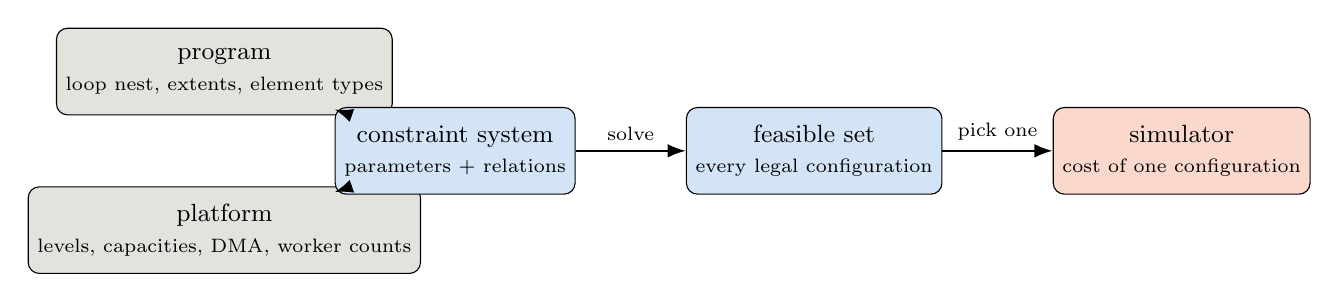
\begin{tikzpicture}[node distance=.9cm and 1.4cm, every node/.style={font=\small, align=center}, box/.style={draw, rounded corners, minimum height=1.1cm, minimum width=2.9cm}]
    \node[box, fill=cgrid] (prog) {program\\ \scriptsize loop nest, extents, element types};
    \node[box, fill=cgrid, below=of prog] (hw) {platform\\ \scriptsize levels, capacities, DMA, worker counts};
    \node[box, fill=cblue!20, right=of $(prog)!.5!(hw)$] (cs) {constraint system\\ \scriptsize parameters + relations};
    \node[box, fill=cblue!20, right=of cs] (feas) {feasible set\\ \scriptsize every legal configuration};
    \node[box, fill=corange!25, right=of feas] (sim) {simulator\\ \scriptsize cost of one configuration};
    \draw[-{Latex}, thick] (prog) -- (cs);
    \draw[-{Latex}, thick] (hw) -- (cs);
    \draw[-{Latex}, thick] (cs) -- node[above, font=\scriptsize] {solve} (feas);
    \draw[-{Latex}, thick] (feas) -- node[above, font=\scriptsize] {pick one} (sim);
  \end{tikzpicture}
  \bigskip
  \begin{columns}[T]
    \column{.45\textwidth}
    \begin{block}{$1024^2$ gemv, one rank}
      Cartesian product \hfill $4.06 \times 10^{9}$\\
      feasible \hfill \textbf{3\,234}\\
      density \hfill $8 \times 10^{-7}$\\
      solved in \hfill 10 ms
    \end{block}
    \column{.45\textwidth}
    % Nothing in the space was written by hand. Swap the platform description and the same derivation yields the space of a different CNM system.
  \end{columns}
\end{frame}

\notebookframe{1}{The design space}{Pick a configuration by hand and simulate it. Then let Cinnamon derive the space and read its constraints. \quad \faClock\ 8 min}

% ─────────────────────────────────────────────────────────────────────────
\section{The landscape}

\begin{frame}{We simulated all 3\,234}
  \begin{columns}[T]
    \column{.6\textwidth}
    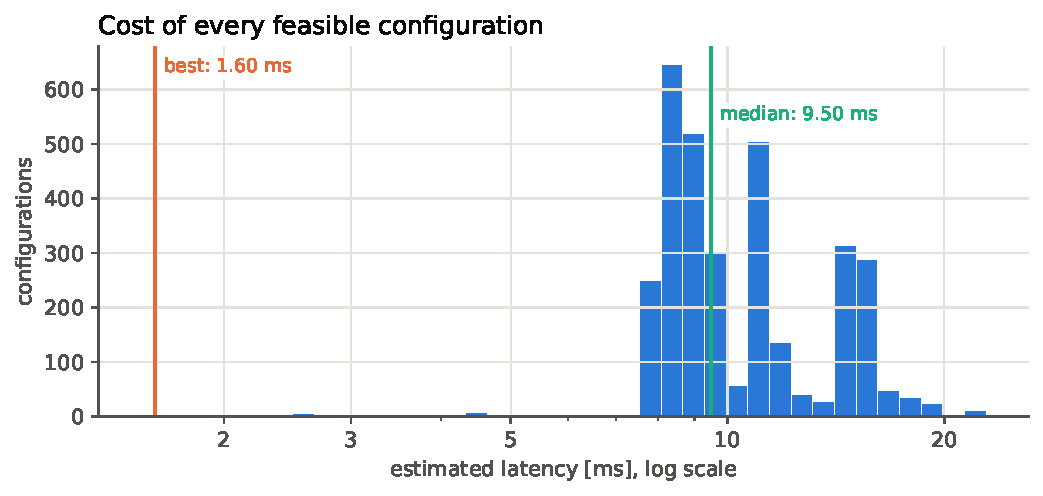
\includegraphics[width=\linewidth]{figures/histogram.pdf}
    \column{.38\textwidth}
    \begin{tabular}{@{}lr@{}}
      \toprule
      best & 1.60 ms \\
      1st percentile & 6.25 ms \\
      median & 9.50 ms \\
      worst & 21.8 ms \\
      \midrule
      within 10\,\% of best & \textbf{6} \\
      within 1.5$\times$ & 11 \\
      within 2$\times$ & 19 \\
      \bottomrule
    \end{tabular}
    \medskip

    The best 0.3\,\% is a separate cluster, $5\times$ below the bulk.
  \end{columns}
\end{frame}

\begin{frame}{Which parameters matter}
  \centering
  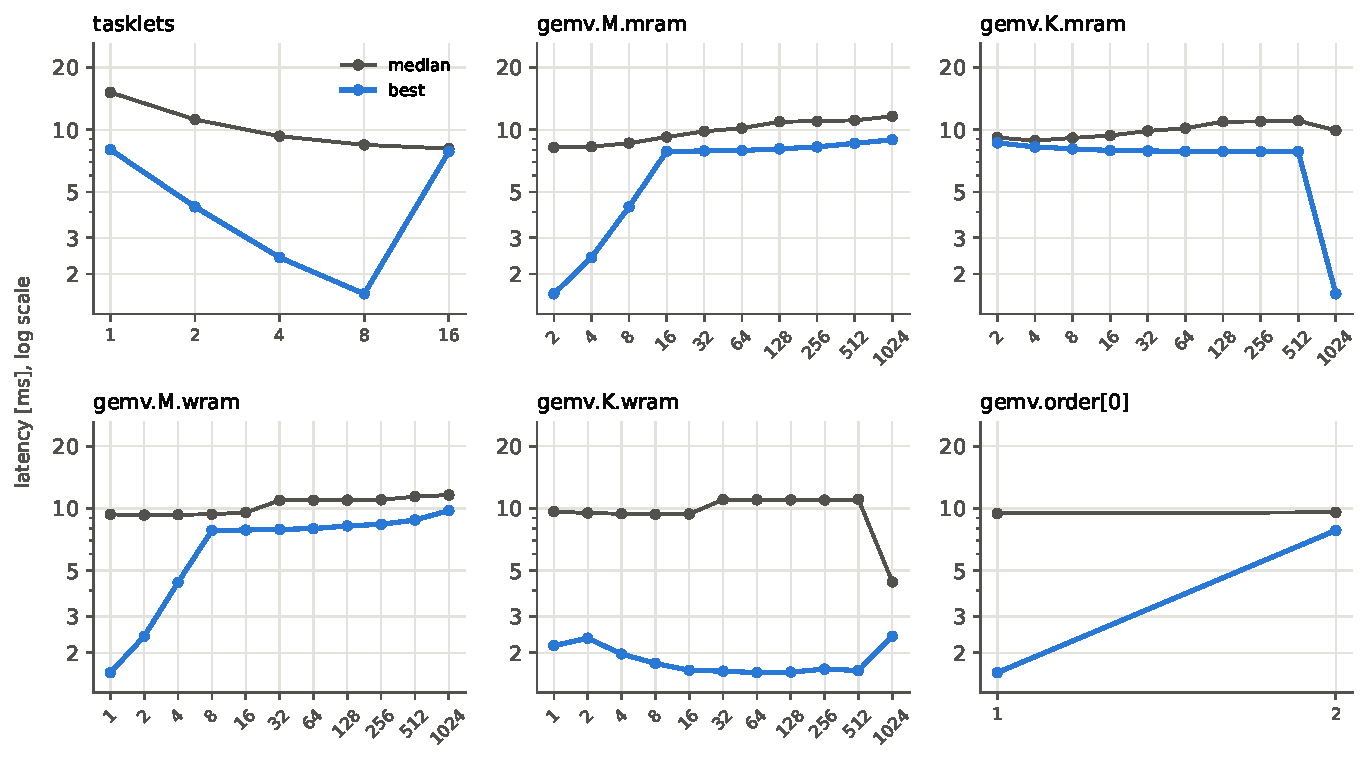
\includegraphics[height=.62\textheight]{figures/marginals.pdf}
  \small\par
  \texttt{tasklets} and \texttt{K.mram} decide everything; the WRAM tiles barely move the best line. \quad The ten best configurations differ in \emph{one} parameter.
\end{frame}

\notebookframe{2}{The landscape}{Where did your guess land? Marginals, the heat map, the top ten. Then pin a hardware knob and search the rest live. \quad \faClock\ 8 min}

% ─────────────────────────────────────────────────────────────────────────
\section{The search}

\begin{frame}{Enumerating is not an option}
  \centering
  \begin{tabular}{@{}lrrr@{}}
    \toprule
    & feasible & one core, fast simulator & \\
    \midrule
    $1024^2$ gemv, 1 rank & 3\,234 & 3 min & \small the oracle you just used \\
    $4096^2$ gemv, 32 ranks & 26\,238 & 1.5 h & \small enumerated once, on 14 cores \\
    $2048^2$ gemm, 32 ranks & 2\,821\,332 & \textbf{47 h} & \small never \\
    \bottomrule
  \end{tabular}
  \bigskip

  \begin{columns}[T]
    \column{.45\textwidth}
    \textbf{Random search} is the honest baseline: no model, no assumptions, and with an oracle it costs nothing to evaluate --- draw from the pool.
    \column{.5\textwidth}
    \textbf{Model-based search} spends simulations where a model says they are worth spending. The question is whether the model learns the landscape faster than random sampling stumbles on it.
  \end{columns}
\end{frame}

\begin{frame}{Bayesian optimisation in one slide}
  \begin{columns}[T]
    \column{.55\textwidth}
    \begin{enumerate}
      \item \textbf{Initial sample} --- a few spread-out configurations, simulated
      \item \textbf{Surrogate} --- fit a model to what was seen; for any configuration it predicts a cost $\mu$ and an uncertainty $\sigma$ \\ \small classically a Gaussian process; here an ensemble of small networks
      \item \textbf{Acquisition} --- score candidates by $\mu - \kappa\sigma$: low predicted cost \emph{or} high uncertainty is attractive
      \item \textbf{Simulate} the best-scoring candidate, add it, go to 2
    \end{enumerate}
    \column{.42\textwidth}
    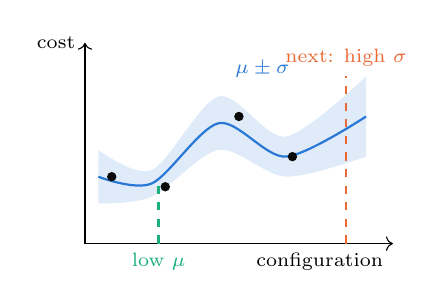
\begin{tikzpicture}[scale=.85, every node/.style={font=\scriptsize}]
      \draw[->] (0,0) -- (4.6,0) node[below left] {configuration};
      \draw[->] (0,0) -- (0,3) node[left] {cost};
      \fill[cblue!15] plot[smooth] coordinates {(0.2,1.4) (1,1.1) (2,2.2) (3,1.6) (4.2,2.5)} -- plot[smooth] coordinates {(4.2,1.3) (3,1.0) (2,1.4) (1,0.7) (0.2,0.6)} -- cycle;
      \draw[cblue, thick] plot[smooth] coordinates {(0.2,1.0) (1,0.9) (2,1.8) (3,1.3) (4.2,1.9)};
      \foreach \x/\y in {0.4/1.0, 1.2/0.85, 2.3/1.9, 3.1/1.3} \fill[cink] (\x,\y) circle (2pt);
      \draw[corange, thick, dashed] (3.9,0) -- (3.9,2.5);
      \node[corange, above] at (3.9,2.5) {next: high $\sigma$};
      \draw[caqua, thick, dashed] (1.1,0) -- (1.1,0.9);
      \node[caqua, below] at (1.1,0) {low $\mu$};
      \node[cblue, right] at (2.1,2.6) {$\mu \pm \sigma$};
    \end{tikzpicture}
  \end{columns}
  \medskip
  \small The infeasible configurations never reach the surrogate: the constraint solver hands it the feasible set, so every simulation is spent on something that can run.
\end{frame}

\notebookframe{3}{The search}{Forty simulations, then five seeds, then a hundred --- each scored against the oracle. Then the space of 26\,238. \quad \faClock\ 9 min}

\begin{frame}{What a budget buys}
  \begin{columns}[T]
    \column{.55\textwidth}
    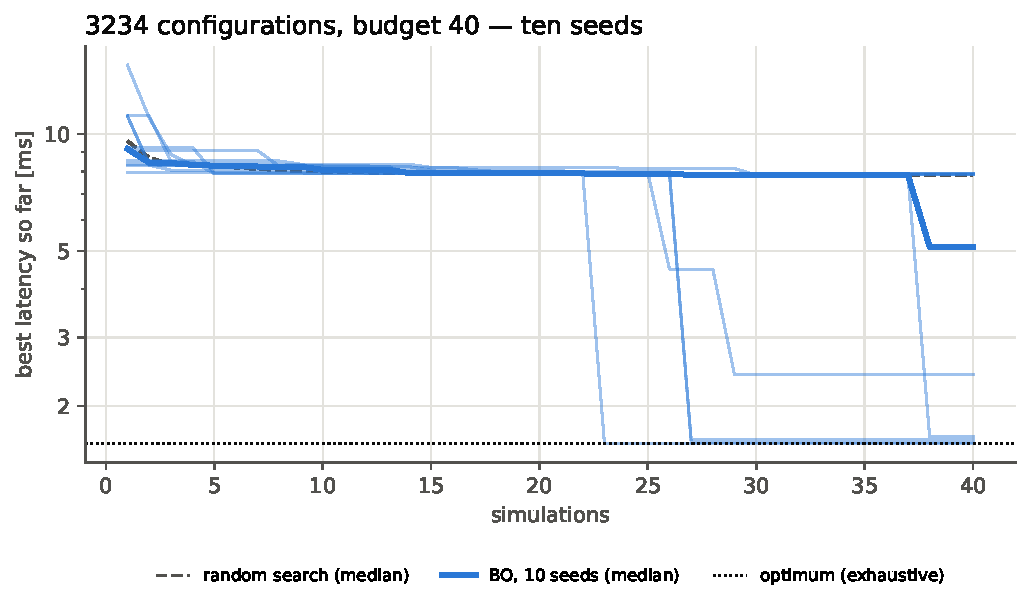
\includegraphics[width=\linewidth]{figures/seeds_small_40.pdf}
    \column{.42\textwidth}
    \textbf{Small space, budget 40, ten seeds}\par\smallskip
    \footnotesize
    \begin{tabular}{@{}rrr@{}}
      \toprule
      seed & best [ms] & rank \\
      \midrule
      166 & 1.60 & 1 \\
      197 & 1.61 & 2 \\
      104 & 1.64 & 4 \\
      290 & 1.67 & 6 \\
      135 & 2.41 & 11 \\
      73 & 7.85 & 45 \\
      259 & 7.87 & 66 \\
      228 & 7.89 & 80 \\
      42 & 7.90 & 103 \\
      321 & 7.91 & 107 \\
      \bottomrule
    \end{tabular}
    \smallskip

    \small Four of ten find the fast line; random search has a 14\,\% chance. With \textbf{budget 100}, four of five seeds land on the exact optimum.
  \end{columns}
\end{frame}

\begin{frame}{Where enumeration was never an option}
  \begin{columns}[T]
    \column{.58\textwidth}
    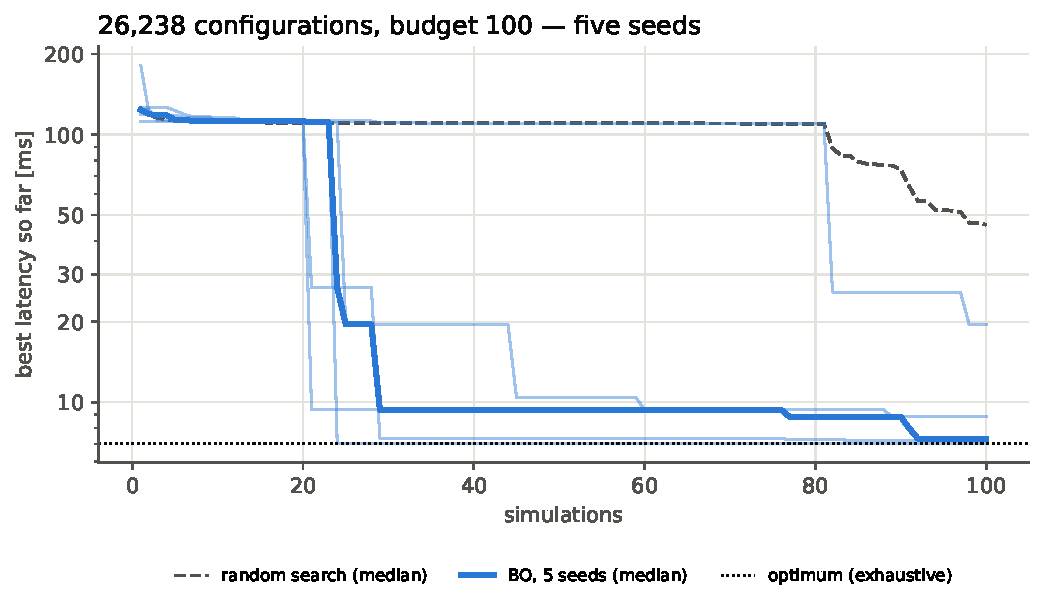
\includegraphics[width=\linewidth]{figures/seeds_big_100.pdf}
    \column{.4\textwidth}
    \textbf{26\,238 configurations, budget 100}\par\smallskip
    \small
    \begin{tabular}{@{}lrr@{}}
      \toprule
      & ms & rank \\
      \midrule
      optimum (oracle) & 7.0 & 1 \\
      Bayesian, best of 5 seeds & 7.0 & 1 \\
      Bayesian, median seed & 7.3 & 8 \\
      Bayesian, worst seed & 19.5 & 82 \\
      random search, median & 46 & \\
      median configuration & 125 & \\
      \bottomrule
    \end{tabular}
    \medskip

    Three of five within 10\,\% of an optimum that only 10 of 26\,238 configurations come within 10\,\% of --- with 0.4\,\% of the simulations.
    \medskip

    \small The 2.8-million space: 60 simulations in 14 s. No oracle --- the two spaces above are its calibration.
  \end{columns}
\end{frame}

% ─────────────────────────────────────────────────────────────────────────
\section{Take-aways}

\begin{frame}{What carries over}
  \begin{enumerate}
    \item \textbf{Derive the space, don't write it.} Program structure $\times$ platform structure $\to$ constraints $\to$ feasible set. The same machinery, another platform description, another system.
    \item \textbf{Hardware knobs live in the same space as the tiling.} Pinning them first caps what any tiling can reach --- and the right pin flips with problem size.
    \item \textbf{Look at the landscape before trusting a search.} Needle or hill, which parameters move the best line, how many configurations are within 10\,\% --- an exhaustive run on a \emph{small} instance answers all three.
    \item \textbf{Score searches against an oracle where you can afford one.} A single run is an anecdote; seeds give a distribution; the oracle gives a regret.
    \item \textbf{Then spend the budget where you cannot.}
  \end{enumerate}
  \bigskip
  \centering\small Cinnamon: \texttt{github.com/tud-ccc/Cinnamon} \quad this tutorial: \texttt{[repository]}
\end{frame}

\end{document}
